\documentclass[conference]{IEEEtran}
\usepackage{cite}
\usepackage{amsmath,amssymb,amsfonts}
\usepackage{graphicx}
\usepackage{textcomp}
\usepackage{xcolor}
\usepackage{booktabs}
\usepackage{multirow}
\usepackage[hidelinks]{hyperref}

\begin{document}

\title{Spectral Signatures of Transformer Redundancy:\\
From Attention-Head Pruning to Embedding Compression}

\author{\IEEEauthorblockN{Sathvik A R}
\IEEEauthorblockA{Department of Computer Science and Engineering\\
PES University, Bengaluru, India\\
\texttt{pes1ug23am275@pesu.pes.edu}}}

\maketitle

\begin{abstract}
Can inexpensive spectral statistics---computed directly from a
transformer's attention maps and embedding parameters with a single
spectral transform---serve as a
\emph{general diagnostic for redundancy}, across both the attention maps
a model computes internally and the embedding tables it stores? We test
this diagnostic hypothesis on head pruning and embedding compression,
and report where it holds, where it fails, and what that boundary teaches.
For pruning, per-head subband statistics rank heads far better than
popular mass heuristics: ranking by attention-map Frobenius norm or
max-column mass is \emph{anti}-predictive of ablation damage at
single-head granularity. A leave-one-cell-out ridge model over these
features is the strongest representation-level predictor we test, keeps
its accuracy when trained \emph{entirely on other architectures}
(leave-one-model-out), and a 45-cell reference sweep confirms the
ordering (87/90 wins vs.\ non-wavelet baselines, all significant under
FDR control). Yet even this most rigorously validated predictor fails
the test that matters: validated downstream, rankings reorder---on
SST-2 the architecture-robust ridge degrades to composite-level
damage while attention-distribution entropy stays safe; on GPT-2 the
asymmetry inverts outright (a different mechanism than the tied-
embedding failure we find on the compression side). Representation-
level screening, however rigorous, does not certify task-level safety.
For compression, an
equal-effective-byte shootout shows int8 quantisation stacks
multiplicatively with frequency-domain sparsification, product
quantization dominates extreme budgets, PCA truncation never wins the
representation-level comparison (though no method is uniformly safe
downstream) ---
and DCT/FFT controls reveal the advantage is generic spectral sparsity
rather than anything wavelet-specific. A downstream transfer study
of compressed tables mirrors the pruning lesson: low degradation on the
tested encoder-classification tasks for every sparse-int8 recipe,
divergent --- even
catastrophic --- under transform-domain coding on the tied-embedding
GPT-2 decoder. Code, evaluation sets and offline
regression tests will be released.
\end{abstract}

\begin{IEEEkeywords}
transformers, attention heads, pruning, spectral analysis, wavelet
transform, model compression, product quantization
\end{IEEEkeywords}

\section{Introduction}
Multi-head self-attention \cite{vaswani2017} accounts for a substantial
share of the parameters and inference cost of modern transformers, and a
large body of evidence shows that many heads are redundant
\cite{michel2019,voita2019,dalvi2020}. Two practical questions follow.
(i)~\emph{Which} heads can be removed safely? Existing answers either
require gradients, behavioural probing, or heuristics---most commonly
the total attention mass a head commands---whose reliability we show is
worse than chance exactly where it matters, in the low-pruning-fraction
regime. (ii)~Once a model is fixed, its token-embedding tables remain a
large dense artifact (e.g., $30{,}522\times768$ float32 $\approx$
90\,MB for BERT); how should they be stored under tight byte budgets?

This paper asks whether the hypothesis survives contact with practice,
and states it as a falsifiable diagnostic claim: \emph{inexpensive
spectral statistics of a representation predict how much redundancy that
representation carries --- and hence what can be removed or compressed
--- uniformly across representation types}. We probe the claim at two
extremes of the redundancy spectrum. Attention maps whose removal is
harmless should look spectrally redundant (concentrated subbands, low
coefficient entropy); token embeddings that survive aggressive lossy
coding should concentrate their information in few spectral components.
The discrete wavelet transform (DWT) \cite{mallat1989,daubechies1992}
supplies the instrument --- one forward pass supplies the attention
maps, the embedding table is read directly, and a linear-time transform
yields signatures that are cheap and training-free ---
and DCT/FFT controls later test whether \emph{wavelets} specifically
matter or whether any frequency-domain basis carries the signal
(\S\ref{sec:compress}). Equally important, we map where the diagnostic
breaks: its rankings are validated at the representation level, and we
show by direct experiment that such validation does not automatically
transfer to task-level damage for either pruning (\S\ref{sec:downstream})
or table compression (\S\ref{sec:compress}).

\textbf{Contributions.}
\begin{enumerate}
\item Per-head wavelet signatures predict single-head ablation damage
significantly better than mass heuristics; Frobenius-mass and
max-column-mass rankings are sign-inverted (anti-predictive) at this
granularity (\S\ref{sec:singlehead}).
\item A seed-replicated local benchmark (nine cells, twelve predictors
including zero-shot proxies of published criteria and a
leave-one-cell-out ridge model) plus
a 45-cell reference sweep across five model families confirm the
representation-level ordering at scale: $87/90$ paired wins over
non-wavelet baselines, all significant (\S\ref{sec:bench},
\S\ref{sec:scale}), and the ridge predictors keep their accuracy when
trained leave-one-model-out (\S\ref{sec:bench}).
\item A downstream-task validation (fine-tuned SST-2 accuracy, GPT-2
perplexity) quantifies the representation-to-task gap for the whole
predictor family: true attention entropy transfers best to SST-2; the
hand-weighted wavelet composite collapses; Frobenius-mass rankings
invert between levels; and even the leave-one-model-out ridge --- the
strongest, most rigorously validated representation-level predictor ---
inherits the gap, showing that learning against representation damage
does not substitute for task-level validation (\S\ref{sec:downstream}).
\item A controlled compression shootout at equal \emph{effective} bytes
shows int8 quantisation stacks multiplicatively with sparsification,
dense product quantization dominates below $\sim$10\% budgets, and PCA
truncation never wins the representation-level comparison; DCT/FFT
controls show the advantage is generic spectral sparsity, and the
residual basis ranking follows table heavy-tailedness
(\S\ref{sec:compress}, \S\ref{sec:gen}). A downstream transfer study of
compressed tables mirrors the pruning lesson and exposes a
tied-embedding failure mode (\S\ref{sec:compress}).
\end{enumerate}

\section{Background and Related Work}
\subsection{Structured attention-head pruning}
Michel et al. \cite{michel2019} showed that many heads can be removed
after training with little effect and that importance varies by layer;
Voita et al. \cite{voita2019} prune with a differentiable regulariser;
Behnke and Heafield \cite{behnke2021} combine lottery-style retraining
with head dropping for machine translation; Lagunas et al.
\cite{lagunas2021} extend block pruning to whole transformers; Sanh et
al. \cite{sanh2020movement} introduce movement pruning during
fine-tuning; Molchanov et al. \cite{molchanov2017} popularised
gradient/Taylor importance criteria. These approaches either modify
training or require dedicated probes. Our predictors read only the
attention maps of the frozen model, and we evaluate them precisely where
practitioners apply them: ranking heads for zero-ablation, validated
both representationally and on downstream tasks.

\subsection{Redundancy and geometry of representations}
Cordonnier et al. \cite{cordonnier2019} observe that heads can converge
to similar query/key roles; Dalvi et al. \cite{dalvi2020} quantify
redundancy among neurons and layers; Ethayarajh \cite{ethayarajh2019}
documents the anisotropic cone geometry of contextual embeddings. Our
static-table measurements add a spectral view: BERT-family vocabularies
are strongly heavy-tailed (excess kurtosis $12.9$--$22.5$), whereas
GPT-2's near-isotropic table (kurtosis $0.13$) behaves differently under
every compression scheme.

\subsection{Compression and quantization}
Product quantization (PQ) \cite{jegou2011} remains central to
billion-scale nearest-neighbour search \cite{johnson2019}, with anisotropic
refinements \cite{guo2020opq}; integer quantisation underpins deployed
inference \cite{jacob2018,dettmers2022}; low-rank adaptation exploits
spectral structure for parameter-efficient tuning \cite{hu2021lora}.
Wavelets have long served signal compression \cite{mallat1989,
daubechies1992}, but have not been benchmarked head-to-head against PCA
truncation, magnitude sparsification and PQ \emph{at equal effective
byte budgets} on transformer embedding tables.

\subsection{Spectral analysis of learned representations}
SVCCA \cite{raghu2017svcca} compares representations via singular
vectors; spectral bias studies \cite{rahaman2019spectral} show networks
learn low frequencies first. Our results extend this line to
\emph{redundancy prediction}: subband statistics forecast what can be
removed.

\section{Method}
\subsection{Wavelet decomposition of embeddings and attention}
Let $x\in\mathbb{R}^{D}$ be a token embedding ($D{=}768$, or $2048$ for
TinyLlama). We symmetrically pad $x$ to the next power of two $n$, apply
a level-$L$ DWT with filter $\psi$ (Haar, DB4, Sym4, Coif2; default DB4),
obtaining approximation coefficients $c_A$ and detail coefficients
$c_{D,\ell}$, $\ell=1..L$ (level 1 = finest), with subband energies
$E_\ell=\lVert c_{D,\ell}\rVert^2$. Attention matrices receive the same
machinery in 2-D (separable DWT2) on the row-normalised matrix, yielding
$(cAH,cAV,cAD)$ subbands per level. Per head we record: total/approx/
low/high-band energies and their ratio (low = coarsest half of levels),
Shannon entropy of normalised coefficient magnitudes, spectral entropy
over level energies, Gini coefficient of magnitudes, reconstruction L2
error after zeroing the smallest 30\% of detail coefficients, and the
coefficient count retaining 99\% energy.

\subsection{Head-importance predictors}
\label{sec:method-pred}
Each predictor maps per-head metrics to a score $s_h$ (higher =
predicted more important / less prunable):
\texttt{wavelet\_entropy} ($s=$ coefficient entropy);
a \texttt{wavelet} composite computed as the raw-scale sum
$e+g+\tfrac12 r+\tfrac12\rho$ over entropy $e$, Gini $g$,
reconstruction error $r$ and energy ratio $\rho$. We emphasise that this
composite mixes unnormalised quantities (entropy spans several bits,
$r$ lives near $10^{-2}$), so its effective weighting is dominated by
$e$; we retain it as the historically specified heuristic and
\emph{treat the ridge models below as its principled counterpart};
\texttt{frobenius\_mass} ($\lVert A\rVert_F$ of the attention map);
\texttt{max\_column\_mass} (mean over rows of each column's maximum);
\texttt{random};
\texttt{attention\_entropy\_true}, the Shannon entropy
$-\sum_q\sum_c p_{qc}\log p_{qc}$ of the attention distribution itself.
For controlled zero-shot comparison we additionally construct three
attention-only \emph{proxies inspired by published criteria}. These are
deliberately \emph{not} reproductions of the original task-aware,
training-time algorithms; they exist so that every method sees exactly
the same inputs under identical conditions:
\texttt{michel\_inspired} follows Michel et al.'s discardability notion
\cite{michel2019} via the magnitude--peakedness proxy
$\lVert A\rVert_F\cdot(1-H(A)/\log T)$ --- heads with near-uniform
attention score as discardable;
\texttt{voita\_inspired} follows Voita et al.'s importance notion
\cite{voita2019} as
$\overline{\max_c A_{\cdot c}}\cdot(1-r)$, i.e.\ kept attention mass
discounted by the 30\%-threshold wavelet reconstruction error $r$; and a
\texttt{behavioural\_similarity} proxy scores each head by behavioural
dissimilarity, $1-\max_{h'\neq h,\,\mathrm{layer}(h')=\mathrm{layer}(h)}
\cos(\mathrm{vec}(A_h),\mathrm{vec}(A_{h'}))$, so redundant near-copies
rank as discardable. All three consume exactly the same per-head
attention maps and metric rows as our predictors. Three ridge regressors
fit on (a) wavelet features only, (b) distributional features only,
(c) both, are trained \emph{leave-one-cell-out} (LOOO): weights for
every held-out cell are fitted on all other cells' (features, measured
loss) pairs; inputs are standardised within each cell; $\alpha{=}1$. The
ridge models answer the composite's weighting problem by learning it.

\subsection{Evaluation protocol and sign convention}
Representation-level ground truth for one input is the per-head cosine
drop between original and ablated sentence representations when head $h$
alone is zero-ablated (hooks on the post-attention projection make this
architecture-agnostic). Stored correlations use
$\mathrm{corr}(-s,\Delta)$ where $\Delta$ is the damage; because batched
pruning removes the \emph{lowest-scored} fraction, a good predictor has
\emph{negative} stored correlations. Orientation-free batched sweeps
(damage vs.\ pruned fraction) complement the correlations.
\emph{Downstream ground truth}: SST-2 validation accuracy for
fine-tuned BERT-base/DistilBERT classifiers and WikiText-2 perplexity
for GPT-2, each re-measured with the bottom-$p\%$ heads (by each
predictor's ranking, computed from sample texts through the same frozen
model) simultaneously ablated.

\subsection{Compression schemes at equal effective bytes}
All methods are compared at equal \emph{total} storage per token:
payload \emph{plus} metadata \emph{plus} amortised shared parameters.
With vocabulary size $V$: PCA/random-projection store $d$ floats
($4d$\,B) plus their projection matrix ($D d\,4/V$; PCA adds a mean row,
$D\,4/V$); sparse variants store kept coefficients as value $+$ uint16
index ($6$\,B fp32, $3$\,B int8 $+$ 2\,B per-vector scale); PQ stores an
$m$-byte code plus the codebook ($256\cdot D\cdot4/V$; $26$\,B/token for
$D{=}768$, $65$\,B/token for $D{=}2048$ at $V{\approx}30$k--50k).
At million-vector deployment scales this amortised overhead falls to
roughly $0.8$--$2.1$\,B/token for $D{=}768$--$2048$, and continues to
decrease with scale.
Quality metrics: cosine between original and reconstructed vectors and
Jaccard overlap of top-10 cosine neighbours before vs.\ after
compression, over 1{,}500 held-out tokens per model (PCA/PQ fitted on a
disjoint split).

\section{Experimental Setup}
\textbf{Models.} bert-base-uncased, distilbert-base-uncased (encoders;
144/72 heads), GPT-2 (decoder; 144 heads); generality sweep adds
RoBERTa-base \cite{liu2019}, DeBERTa-base \cite{he2021} and
TinyLlama-1.1B \cite{zhang2024} ($D{=}2048$).
\textbf{Data.} Static tables: full HF vocabularies. Contextual probe: a
10-anchor polysemy set. Attention/pruning: a curated 12-sentence eval
set spanning polysemy, relative clauses, passives, named entities,
numerals, questions; benchmark corpus: WikiText-2 sentences
\cite{merity2017} filtered to clean single sentences ($\approx$70k pool).
\textbf{Downstream.} textattack/bert-base-uncased-SST-2 and
distilbert-base-uncased-finetuned-sst-2-english on GLUE SST-2
validation (872 examples); GPT-2 perplexity on the WikiText-2 test split.
\textbf{Hardware.} All experiments run CPU-only (Intel i7-1355U); the
pipeline supports containerised GPU sweeps.
\textbf{Statistics.} Paired Wilcoxon tests, Cohen's $d$, Cliff's
$\delta$, bootstrap CIs, three seeds per cell. Where multiple paired
comparisons are reported together we additionally apply
Benjamini--Hochberg false-discovery-rate control at $\alpha{=}0.05$.
\textbf{Unit of analysis.} Every paired test operates on \emph{per-input
correlation values} --- one Pearson $r$ per sentence input, computed over
all heads of that input --- so the sample entering a Wilcoxon test is the
set of inputs ($n{=}12$ per local cell, $150$ per reference-sweep cell
group), never individual heads (heads within one network are strongly
dependent). The three seeds contribute disjoint sentence subsets drawn
without replacement from the cleaned corpus, so pooling seeds widens
coverage without duplicating inputs; seed-level variance is reported
separately.

\section{Results}
\subsection{Static spectra differentiate model families}
BERT/DistilBERT vocabularies are strongly heavy-tailed (excess kurtosis
$12.9$/$22.5$, skew $-1.95$/$-2.97$) while GPT-2's are near-Gaussian
(kurtosis $0.13$); mean embedding energy differs by $8\times$
($21.1$ vs.\ $2.6$). Energy concentrates in the finest bands (low/high
ratios $0.15$--$0.55$): token identity lives in high-frequency detail.
Zeroing the smallest 10\%/50\% of detail coefficients reconstructs at
cosine $\geq0.999$/$\geq0.964$.

\subsection{Spectral signatures track word sense}
On the polysemy probe (DistilBERT, DB4), cross-sense spectrum separation
tracks raw-cosine separation (bank $0.234$ vs.\ $0.222$) and same-sense
similarity exceeds cross-sense similarity for all ten anchors
(inter $0.56$--$0.84$ vs.\ cross $0.29$--$0.68$): spectra are
sense-sensitive, though not more discriminative than cosine here.

\subsection{Layer progression}
Across DistilBERT layers, the low/high-frequency energy ratio rises
($1.35\rightarrow2.03$), Gini grows ($0.57\rightarrow0.71$), entropy
falls ($7.16\rightarrow6.60$ bits) and 30\%-threshold reconstruction
error halves ($0.059\rightarrow0.028$): later layers attend through
fewer, lower-frequency, more compressible patterns.

\subsection{Single-head prediction: mass heuristics are anti-predictive}
\label{sec:singlehead}
Table~\ref{tab:singlehead} reports stored correlations (negative =
better). The wavelet composite and true attention entropy form the best
tier; \emph{Frobenius mass} and \emph{max-column mass} carry positive
correlations: their lowest-scored heads are the \emph{most} damaging to
remove. The orientation-free bottom-10\% sweep makes this concrete ---
damage under lowest-score-first pruning:
$0.00056$ (attn-entropy-true), $0.00072$ (wavelet),
$0.00077$ (wavelet-entropy), $0.00256$ (random), $0.00318$
(Frobenius mass), $0.00481$ (max-column mass). Ranking by
$\lVert A\rVert_F$---a common shortcut---is $4.4\times$ worse than
random here.

\begin{table}[t]
\centering
\caption{Single-head pruning prediction (stored Pearson
$r=\mathrm{corr}(-s,\Delta)$; more negative = better). DB4,
12-sentence eval set. The GPT-2 column is computed on a near-null
damage signal (single-head drops ${\sim}10^{-4}$) and should be read
as a noise floor rather than a ranking.}
\label{tab:singlehead}
\begin{tabular}{lrrr}
\toprule
Predictor & BERT-base & DistilBERT & GPT-2 \\
\midrule
Attn.\ entropy (true) & $-0.32$ & $\mathbf{-0.40}$ & $-0.14$ \\
Wavelet composite     & $\mathbf{-0.31}$ & $-0.33$ & $-0.16$ \\
Wavelet entropy       & $-0.14$ & $-0.02$ & $-0.18$ \\
Random                & $-0.02$ & $+0.30$ & $-0.02$ \\
Frobenius mass $\lVert A\rVert_F$ & $+0.33$ & $+0.39$ & $+0.16$ \\
Max-column mass       & $+0.33$ & $+0.36$ & $+0.19$ \\
\bottomrule
\end{tabular}
\end{table}

In batched bottom-$p\%$ sweeps (Fig.~\ref{fig:prune}) the wavelet
composite is best-or-tied-best in 5/12 model$\times$ratio cells and
never worse than random; the attention-entropy family wins most other
cells. GPT-2 is nearly insensitive to single-head ablation at this probe
(drops ${\sim}10^{-4}$), compressing all differences there.

\begin{figure}[t]
\centering
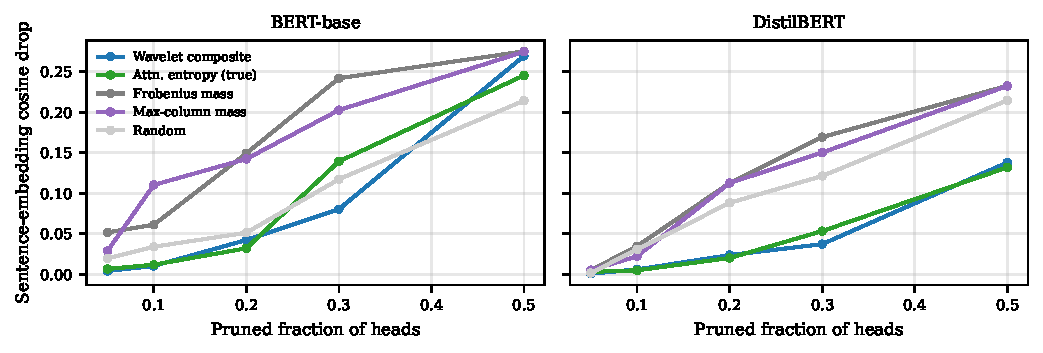
\includegraphics[width=\linewidth]{figs/pruning_sweep.pdf}
\caption{Batched fairness sweep: mean sentence-representation cosine
drop after ablating the bottom $p\%$ of heads ranked by each predictor
(DB4, encoder models). Lower is safer.}
\label{fig:prune}
\end{figure}

\subsection{Seed-replicated benchmark with learned combination}
\label{sec:bench}
Across nine (model, dataset, seed) cells on WikiText-2 sentences
(Table~\ref{tab:bench}), the \emph{learned} predictors lead: the LOOO
ridge over combined features is the best overall predictor on DistilBERT
($-0.41$), the wavelet-only ridge is best on BERT-base ($-0.328$), and
the combined model statistically ties wavelet-only there ($+0.007$,
$p=0.30$) while lifting significantly over it on DistilBERT
($\Delta=-0.074$, $p=5\times10^{-4}$). Against every non-learned
comparator --- mass heuristics and published-criterion-inspired proxies
alike --- the combined model wins with $p\leq0.0024$ and $|d|$ up to
$9$ on both encoders. Wavelet-side rankings beat the comparators in
72/105
comparisons overall. Seed standard deviation is non-degenerate
($0.003$--$0.048$). We report the hand-weighted composite for continuity
with the specification it came from, but treat the ridge models --- which
learn the weighting from data with no test-cell leakage --- as the
primary wavelet-feature predictors throughout.

\emph{Leave-one-model-out transfer.} Because cells sharing a model may
correlate, we re-fit the ridges under a harsher protocol: all weights
are learned from the \emph{other two architectures only} and applied to
every input of the held-out model. Cross-architecture transfer holds:
the combined ridge reaches mean stored $r=-0.28/-0.40/-0.23$ on
held-out BERT/DistilBERT/GPT-2 (vs.\ $-0.32/-0.41/-0.15$ when its own
architecture's other seeds assist training), and wavelet-only features
transfer at $-0.28/-0.34/-0.27$. The ordering of predictors is
unchanged under this protocol; only GPT-2's absolute values shift
appreciably, consistent with its near-null damage signal.

\begin{table}[t]
\centering
\caption{Local benchmark mean stored correlations (more negative =
better; WikiText-2, seeds $\{0,1,2\}$, 12 inputs/cell).}
\label{tab:bench}
\begin{tabular}{lrrr}
\toprule
Predictor & BERT-base & DistilBERT & GPT-2 \\
\midrule
\textbf{Ridge: combined}        & $-0.320$ & $\mathbf{-0.413}$ & $-0.153$ \\
\textbf{Ridge: wavelet-only}    & $\mathbf{-0.328}$ & $-0.338$ & $-0.189$ \\
\textbf{Ridge: attn.-only}      & $-0.237$ & $-0.327$ & $-0.219$ \\
Attn.\ entropy (true)           & $-0.237$ & $-0.327$ & $\mathbf{-0.219}$ \\
Wavelet entropy                 & $-0.203$ & $-0.125$ & $-0.154$ \\
Wavelet composite (heuristic)   & $-0.117$ & $-0.130$ & $-0.213$ \\
Frobenius mass                  & $+0.256$ & $+0.332$ & $+0.221$ \\
Max-column mass                 & $+0.270$ & $+0.332$ & $+0.227$ \\
Random                          & $+0.031$ & $+0.278$ & $-0.048$ \\
\bottomrule
\end{tabular}
\end{table}

\subsection{Scale validation: 45-cell reference sweep}
\label{sec:scale}
To address small-sample concerns we report a larger reference run
executed on containerised GPUs: $45$ cells $=$ five model families
(BERT-base, DistilBERT, GPT-2, RoBERTa-base, TinyLlama) $\times$ three
corpora (WikiText-2, Penn Treebank, GLUE subset) $\times$ three seeds,
with $150$ inputs per cell group and the fixed non-ridge predictor set
described in \S\ref{sec:method-pred}.
The strength of this sweep lies less in any single p-value than in the
convergence of evidence: five architectures, three corpora, disjoint
per-seed inputs, and rankings that agree with the small-scale study.
Table~\ref{tab:gpusweep} pools dataset-level means per model. In the
$90$ paired comparisons between the two wavelet-side scores
(composite, coefficient entropy) and the five non-wavelet baselines
(Frobenius mass, max-column mass, random, Michel-/Voita-inspired
proxies),
the wavelet side is better in $\mathbf{87/90}$ and \emph{all 90} are
statistically significant (Wilcoxon; every one survives
Benjamini--Hochberg FDR control at $\alpha{=}0.05$, largest raw
$p=10^{-5}$). Across all $105$ pairwise comparisons recorded by the
harness, the wavelet side wins $91$, with $103$ significant
($103/105$ under BH-FDR). Seed standard deviations span
$0.0001$--$0.0124$. Two honest caveats: DeBERTa cells were produced
before the architecture-agnostic ablation hook covered disentangled
attention and are excluded; on TinyLlama the behavioural-similarity
proxy is anomalously strong ($-0.32$), the only case where a
non-wavelet-side ranking leads.

\begin{table}[t]
\centering
\caption{Reference sweep (45 cells, GPU): pooled mean stored
correlations per model family (more negative = better).}
\label{tab:gpusweep}
\setlength{\tabcolsep}{3.4pt}
\begin{tabular}{lrrrrr}
\toprule
Model & Wavelet & Coeff.-ent. & Frob. & ColMass & Rand. \\
\midrule
BERT-base   & $-0.136$ & $-0.238$ & $+0.254$ & $+0.262$ & $-0.003$ \\
DistilBERT  & $-0.123$ & $-0.172$ & $+0.325$ & $+0.321$ & $+0.279$ \\
GPT-2       & $-0.224$ & $-0.169$ & $+0.226$ & $+0.230$ & $-0.050$ \\
RoBERTa     & $-0.138$ & $-0.235$ & $+0.155$ & $+0.140$ & $-0.039$ \\
TinyLlama   & $-0.216$ & $-0.228$ & $+0.178$ & $+0.183$ & $-0.006$ \\
\bottomrule
\end{tabular}
\end{table}

\subsection{Downstream task validation}
\label{sec:downstream}
Table~\ref{tab:downstream} re-ranks the same predictors by
\emph{task}-level damage, and the picture inverts across objectives.
On SST-2, true attention entropy is the most robust ranking (bottom-30\%
pruning costs $11.2$/$5.9$ accuracy points on BERT/DistilBERT), while
the wavelet \emph{composite} --- strong at representation level ---
collapses ($+41.5$/$+42.0$ points). On GPT-2 perplexity the ordering
flips entirely: the wavelet composite is by far the safest ranking
(perplexity $1.25\times$/$2.7\times$/$3.3\times$ clean at 10/20/30\%,
vs.\ random at $12.8\times$/$62\times$/$39.5\times$), whereas attention
entropy becomes catastrophic ($1.9\times$/$32.7\times$/$160\times$).
Frobenius mass is likewise level-inconsistent: anti-predictive for
representation damage yet among the best SST-2 rankings on DistilBERT
($+0.6/+1.3/+4.9$ points). Most tellingly, the entire \emph{learned}
ridge family --- our strongest representation-level predictors under
both LOOO and leave-one-model-out training --- degrades downstream:
the combined ridge loses $14.3/41.2/41.5$ accuracy points on BERT, and
even its attn-only variant, the gentlest learned ranking, tracks
attention entropy rather than beating it. Learning the feature weighting
against representation damage does not repair objective mismatch: an
estimator optimised for that damage inherits its blind spots. The GPT-2
column adds an instructive asymmetry. The plain wavelet composite is the
safest ranking there ($1.3\times$/$2.7\times$/$3.3\times$), yet the
ridge fitted \emph{on wavelet features alone} is far worse
($18\times$/$12\times$/$29\times$): fitting weights to
representation-level loss destroyed whatever accidental alignment made
the composite robust. Conversely the attn-only ridge hedges attention
entropy's blow-up ($2.6\times$/$3.0\times$/$5.8\times$ vs.\ $160\times$
at 30\%) by diluting it with other features. Mixing hedges; it does not
compose. Two conclusions follow. First,
representation-level cosine damage is an imperfect proxy: predictor
rankings reorder across downstream objectives and architectures --- even
when the predictor is learned against that proxy under rigorous
protocols --- so any pruning claim must include a task-level check
matched to the deployment objective. Second, the right target for
learned rankers is the damage metric a practitioner actually cares
about: fit ridges on task-level losses directly.

\begin{table*}[t]
\centering
\caption{Downstream-task validation: damage after pruning the
bottom-$p$\% of heads ranked by each predictor. Accuracy drops
(points) and perplexity ratios ($\times$ clean) computed against
each model's unpruned score; lower is better. No predictor
dominates: distributional entropy transfers best to SST-2 but
collapses on GPT-2, where the wavelet composite excels ---
task-level validation is indispensable.}
\label{tab:downstream}
\begin{tabular}{lrrrrrrrrr}
\toprule
 & \multicolumn{3}{c}{BERT SST-2 $\Delta$acc.} & \multicolumn{3}{c}{DistilBERT SST-2 $\Delta$acc.} & \multicolumn{3}{c}{GPT-2 PPL ratio} \\
Predictor & 10\% & 20\% & 30\% & 10\% & 20\% & 30\% & 10\% & 20\% & 30\% \\
\midrule
Wavelet composite & +8.9 & +35.6 & +41.5 & +6.5 & +14.4 & +42.0 & 1.25 & 2.66 & 3.26 \\
Attn.\ entropy (true) & +1.2 & +6.3 & +11.2 & +1.4 & +5.4 & +5.8 & 1.91 & 32.65 & 159.53 \\
Frobenius mass $\|A\|_F$ & +6.4 & +5.5 & +16.2 & +0.6 & +1.3 & +4.9 & 2.39 & 5.15 & 6.43 \\
Max-column mass & +1.8 & +14.1 & +18.8 & +0.9 & +1.8 & +10.8 & 2.23 & 5.05 & 8.40 \\
Random & +4.8 & +39.0 & +41.5 & +4.0 & +15.0 & +42.0 & 12.75 & 61.99 & 39.49 \\
Ridge: wavelet-only (LOMO) & +15.7 & +41.5 & +41.5 & +7.7 & +42.0 & +42.0 & 18.31 & 11.67 & 28.84 \\
Ridge: attn.-only (LOMO) & +5.7 & +10.6 & +11.2 & +0.1 & +2.8 & +3.7 & 2.57 & 2.99 & 5.84 \\
Ridge: combined (LOMO) & +14.3 & +41.2 & +41.5 & +6.5 & +22.8 & +42.0 & 7.81 & 16.25 & 23.70 \\
\midrule
Clean model & 92.4 & -- & -- & 91.1 & -- & -- & 39.4 & -- & -- \\
\bottomrule
\end{tabular}
\end{table*}


\subsection{Compression at equal effective bytes}
\label{sec:compress}
Fig.~\ref{fig:compress} and Table~\ref{tab:effbytes} compare methods at
equal \emph{total} storage. Three effects survive the stricter
accounting.
(i)~\emph{int8 stacks}: at matched bytes the int8 twin of a
sparsifier keeps $2\times$ more coefficients than its fp32 counterpart
for identical bytes and dominates everywhere
(e.g., 1024\,B: $0.95$ vs.\ $0.83$ cosine for raw top-k).
(ii)~\emph{PQ owns the extreme regime}: at $128$ effective bytes/token
($24\times$ smaller than the original payload) it reconstructs at
cosine $0.88$ retaining $41$\% of exact top-10 neighbours; no per-vector
method exceeds $0.54$ there. Its codebook amortisation ($26$--$65$\,B/
token at these vocabulary sizes) is included; at million-vector
deployment scales the overhead falls to roughly $0.8$--$2.1$\,B/token
for $D{=}768$--$2048$, and its advantage widens further.
(iii)~\emph{PCA never wins}: global principal components align poorly
with per-token information; even untrained random projection is often
competitive, and both trail sparsification except at saturating budgets.
(iv)~\emph{The sparse-coding advantage is largely generic spectral
sparsity, not wavelet-specific}: adding DCT-II (global frequency basis,
no multiresolution) and rFFT controls at identical coefficient counts
and byte charges, the DCT tracks or exceeds the DB4 wavelet column on
cosine at every effective budget (pooled over six models, fp32
payloads: $0.50$/$0.59$/$0.70$ vs.\ wavelet $0.44$/$0.58$/$0.69$ at
128/256/512\,B), with neighbour overlap statistically indistinguishable,
and the complex-valued FFT trailing both only because its payload costs
more per kept coefficient. Within transform-domain sparsification, the
choice of orthonormal frequency basis contributes little; multiresolution
itself provides no measurable advantage for fixed-length embedding
vectors.
The wavelet-vs-raw-topk question is decided by table geometry
(\S\ref{sec:gen}), and the DCT/FFT controls bound how much of that is
\emph{wavelet}-specific: little.

\emph{From representation metrics to tasks.} Applying the same lesson we
learned for pruning, we replace each model's word-embedding table with
its lossy reconstruction and re-measure the task metric
(Table~\ref{tab:dscomp}). On the fine-tuned SST-2 classifiers,
\emph{every} tested int8 sparsification recipe --- wavelet, DCT, and
raw coordinate top-k alike --- transfers with low degradation (all
drops $\leq4.9$ points at 17\% and $\leq0.7$ points at 33\%), confirming
that the
strong representation-level performance of sparse int8 coding transfers
to these encoder tasks \emph{without a unique advantage for the
spectral bases}. At 33\% storage every tested sparse-int8 method stays
within 0.7 accuracy points on both encoders; at 17\%, degradation
remains modest but reaches 4.9 points. PCA truncation at matched effective bytes is
dramatically worse ($-36$/$-17$ points at 33\%) despite respectable
cosine --- exactly the representation-vs-task gap the pruning study
exposed, now on the compression side. GPT-2 is harsher still, and here
the bases separate: wavelet and DCT tables diverge outright
($>10^{3}\times$ clean perplexity), PCA leaves $22$--$47\times$
degradation, while \emph{raw-coordinate} top-k int8 at the 33\% budget
survives at $1.21\times$. We hypothesise two mechanisms: GPT-2's
\emph{tied} input/output embedding matrix ($wte$ doubles as the output
softmax weight, so table noise flows straight into every logit)
amplifies any transform that smears perturbations across all
dimensions, whereas coordinate-space selection leaves each surviving
embedding row individually intact. Untying/re-calibration experiments
are left to future work. The practical consequence, stated with its
scope: in the two encoder-classification settings tested, every tested
int8 sparsification recipe transfers with little task degradation
regardless of basis, while tied decoder tables require basis-aware
choices and separate task-level validation --- representation-level
metrics alone would have hidden every one of these failures.

\begin{table*}[t]
\centering
\small
\caption{Downstream validation of embedding-table
compression: the word-embedding matrix is replaced by its
lossy reconstruction (int8 payloads; PCA dense) and the task
metric re-measured. Accuracy drops (points) and perplexity
ratios ($\times$ clean); lower is better. On both encoder
classifiers every tested int8 sparsification recipe --- wavelet,
DCT, and raw top-k alike --- transfers with low degradation, and
is near-lossless at the 33\% budget --- while PCA
truncation does not. On tied-embedding GPT-2 the transform-domain
tables fail catastrophically at both budgets while raw-coordinate
TopK stays robust at 33\% ($1.2\times$): where a perturbation
lands can matter more than how close the reconstruction is.}
\label{tab:dscomp}
\begin{tabular}{lcccccccc}
\toprule
 & \multicolumn{2}{c}{Wav.+int8} & \multicolumn{2}{c}{DCT+int8} & \multicolumn{2}{c}{TopK+int8} & \multicolumn{2}{c}{PCA} \\
Model & 17\% & 33\% & 17\% & 33\% & 17\% & 33\% & 17\% & 33\% \\
\midrule
BERT SST-2 & +1.9 & +0.3 & +0.7 & +0.3 & +0.8 & +0.6 & +39.0 & +36.0 \\
DistilBERT SST-2 & +4.9 & +0.1 & +1.1 & +0.7 & +1.5 & +0.5 & +25.2 & +17.1 \\
GPT-2 PPL & $>$1000$\times$ & $>$1000$\times$ & $>$1000$\times$ & $>$1000$\times$ & $>$1000$\times$ & 1.2$\times$ & 46.7$\times$ & 21.6$\times$ \\
\bottomrule
\end{tabular}
\end{table*}


\begin{figure}[t]
\centering
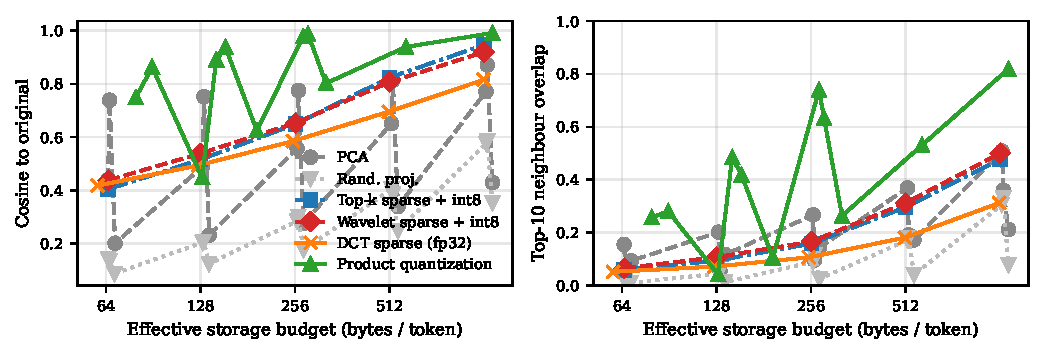
\includegraphics[width=\linewidth]{figs/compression_shootout.pdf}
\caption{Compression quality vs.\ effective storage budget
(bytes/token including metadata and amortised shared parameters;
original $=3072$\,B for $D{=}768$). Pooled over six models.}
\label{fig:compress}
\end{figure}

\begin{table}[t]
\centering
\caption{Equal-\emph{effective}-byte comparison pooled over six models
(cosine / top-10 neighbour Jaccard). Best sparse method per row
bolded.}
\label{tab:effbytes}
\setlength{\tabcolsep}{3.0pt}
\begin{tabular}{rrrrrr}
\toprule
$B_{\mathrm{eff}}$ & PCA & Rand.proj. & TopK-int8 & Wav-int8 & PQ \\
\midrule
128  & $.53/.14$ & $.19/.04$ & $.52/.09$ & $.54/\mathbf{.11}$ &
$\mathbf{.88/.41}$ \\
192  & $.56/.17$ & $.24/.07$ & $.59/.13$ & $.61/\mathbf{.14}$ &
$\mathbf{.89/.48}$ \\
256  & $.58/.19$ & $.27/.09$ & $.65/.16$ & $.65/\mathbf{.17}$ &
$\mathbf{.93/.59}$ \\
384  & $.69/.25$ & $.35/.14$ & $.76/\mathbf{.25}$ & $.76/\mathbf{.25}$ &
-- \\
512  & $.72/.30$ & $.39/.17$ & $\mathbf{.82/.30}$ & $.81/\mathbf{.31}$ &
-- \\
1024 & $.81/.44$ & $.58/.31$ & $\mathbf{.95}/.48$ & $.92/\mathbf{.50}$ &
-- \\
\bottomrule
\end{tabular}
\end{table}

\subsection{Generalisation to other architectures}
\label{sec:gen}
Repeating the shootout on RoBERTa-base, DeBERTa-base and TinyLlama
($2048$-dim decoder; Table~\ref{tab:gen}), two orderings generalise
universally and one is conditional: int8 stacking strictly dominates its
fp32 twin on every model at every budget; PQ dominates the extreme
regime on every model; PCA never wins overall. Conditionally, spectral
sparsification (wavelet or DCT alike) beats naive coordinate-space
magnitude selection most clearly on the heavy-tailed BERT-family tables,
while on isotropic tables (RoBERTa, DeBERTa, TinyLlama) raw top-k with
int8 payloads becomes the stronger sparse method, and the residual
wavelet-vs-DCT gap is within noise. Heavy-tailedness is measurable in
one pass over a sample, giving practitioners a decision rule for basis
choice --- though given \S\ref{sec:compress}, the safer summary is that
basis choice is secondary to selecting a sparsification strategy
matched to the geometry and downstream use of the embedding table. In
Table~\ref{tab:gen}, ``--'' marks budgets a method cannot meet (for PQ
on TinyLlama, the code plus the amortised codebook exceeds the
128\,B/token budget for every evaluated configuration) or points
outside the evaluated range.

\begin{table}[t]
\centering
\caption{Generalisation of the compression ranking to unseen
architectures at equal \emph{effective} storage budgets
(cosine / top-10 neighbour overlap; bytes/token including all
metadata and amortised shared parameters). Best sparse method
per row bolded; -- = method cannot fit the budget.}
\label{tab:gen}
\begin{tabular}{llrrrr}
\toprule
Model & $B_{\mathrm{eff}}$ & PCA & TopK-int8 & Wav-int8 & PQ \\
\midrule
RoBERTa-base & 128 & 0.42/0.23 & \textbf{0.55/0.13} & 0.48/0.07 & 0.85/0.44 \\
 & 256 & 0.50/0.29 & \textbf{0.69/0.26} & 0.62/0.16 & 0.97/0.72 \\
 & 512 & 0.62/0.39 & \textbf{0.85/0.45} & 0.77/0.31 & -- \\
\midrule
DeBERTa-base & 128 & 0.44/0.22 & \textbf{0.54/0.10} & 0.49/0.07 & 0.85/0.43 \\
 & 256 & 0.52/0.28 & \textbf{0.68/0.19} & 0.63/0.13 & 0.97/0.71 \\
 & 512 & 0.62/0.37 & \textbf{0.83/0.37} & 0.77/0.29 & -- \\
\midrule
TinyLlama-2048 & 128 & 0.23/0.11 & \textbf{0.39/0.04} & 0.36/0.03 & -- \\
 & 256 & 0.27/0.14 & \textbf{0.50/0.07} & 0.48/0.05 & 0.72/0.19 \\
 & 512 & 0.33/0.17 & \textbf{0.63/0.12} & 0.62/0.10 & 0.91/0.48 \\
\bottomrule
\end{tabular}
\end{table}


\section{Limitations}
Our pruning ground truth is representational (sentence-embedding cosine
drop) \emph{and} behavioural (SST-2 accuracy, language-model perplexity),
but the behavioural set covers one classification task and one LM
evaluation; broader task suites may reorder predictors again. The
45-cell reference sweep used the fixed non-ridge predictor set (no LOOO
ridge)
and excludes DeBERTa (its cells predate the architecture-agnostic
ablation hook); DeBERTa appears only in the compression sweep. Local
benchmark cells contain twelve inputs each; we mitigate with seeds,
paired tests and the large reference sweep, but absolute correlation
magnitudes at this scale should be read cautiously. GPT-2's insensitivity
to single-head ablation bounds any predictor's measurable advantage
there. The leave-one-model-out ridge study covers three architectures;
extending it to the five-family scale is future work. Finally, PQ
requires training data and fixed codebooks; for streaming single-vector
storage, sparse int8 coding remains the recommended operating regime,
with the sparsification basis selected according to table geometry and
downstream use --- subject to the tied-embedding caveat of
\S\ref{sec:compress}.

\section{Conclusion}
We asked whether inexpensive spectral statistics act as a general
redundancy diagnostic across transformer representations. The answer is
a qualified yes with a sharp boundary. As a \emph{diagnostic}, spectral
signatures rank attention heads for pruning far better than mass
heuristics (which are anti-predictive at single-head granularity),
transfer across architectures under leave-one-model-out training, and
hold at 45-cell scale; on the compression side they characterise which
sparsification formats perform best at the representation level across
effective budgets, with
DCT/FFT controls showing the effect is generic spectral sparsity rather
than something unique to wavelets. As a \emph{deployment criterion}, the
diagnostic is insufficient --- by design it measures representation
damage, and our downstream studies show rankings reorder between that
objective and task accuracy or perplexity, with catastrophic failures
observed on the tied-embedding GPT-2 decoder --- and they do so
even when the ranking is \emph{learned} against representation-level
damage rather than hand-tuned. Spectral
pre-screening plus task-level validation is therefore the recommended
workflow. Code, evaluation sets and offline regression tests will be
released upon publication.

\begin{thebibliography}{27}

\bibitem{vaswani2017}
A.~Vaswani, N.~Shazeer, N.~Parmar, J.~Uszkoreit, L.~Jones, A.~N. Gomez,
{\L}.~Kaiser, and I.~Polosukhin, ``Attention is all you need,'' in
\emph{Advances in Neural Information Processing Systems}, 2017,
pp. 5998--6008.

\bibitem{devlin2019}
J.~Devlin, M.-W. Chang, K.~Lee, and K.~Toutanova, ``BERT: Pre-training of
deep bidirectional transformers for language understanding,'' in
\emph{Proc. NAACL-HLT}, 2019, pp. 4171--4186.

\bibitem{radford2019}
A.~Radford, J.~Wu, R.~Child, D.~Luan, D.~Amodei, and I.~Sutskever,
``Language models are unsupervised multitask learners,'' OpenAI,
Tech. Rep., 2019.

\bibitem{sanh2019}
V.~Sanh, L.~Debut, J.~Chaumond, and T.~Wolf, ``DistilBERT, a distilled
version of BERT: smaller, faster, cheaper and lighter,'' in
\emph{NeurIPS EMC$^2$ Workshop}, 2019.

\bibitem{michel2019}
P.~Michel, O.~Levy, and G.~Neubig, ``Are sixteen heads really better than
one?'' in \emph{Advances in Neural Information Processing Systems},
2019, pp. 14\,014--14\,024.

\bibitem{voita2019}
E.~Voita, D.~Talbot, F.~Moiseev, R.~Sennrich, and I.~Titov, ``Analyzing
multi-head self-attention: Specialized heads do the heavy lifting, the
rest can be pruned,'' in \emph{Proc. ACL}, 2019, pp. 5797--5808.

\bibitem{behnke2021}
M.~Behnke and M.~Heafield, ``Losing heads in the lottery: Pruning
transformer attention in neural machine translation,'' in
\emph{Proc. EMNLP-IJCNLP}, 2021, pp. 4942--4952.

\bibitem{lagunas2021}
F.~Lagunas, E.~Charlaix, V.~Sanh, and A.~M. Rush, ``Block pruning for
faster transformers,'' in \emph{Findings of EMNLP}, 2021,
pp. 3578--3595.

\bibitem{sanh2020movement}
V.~Sanh, T.~Wolf, and A.~M. Rush, ``Movement pruning: Adaptive sparsity
by fine-tuning,'' in \emph{Advances in Neural Information Processing
Systems}, 2020, pp. 20\,378--20\,389.

\bibitem{molchanov2017}
D.~Molchanov, S.~Tarreev, and J.~Kautz, ``Pruning convolutional neural
networks for efficient inference,'' in \emph{Proc. ICML}, 2017,
pp. 2610--2619.

\bibitem{cordonnier2019}
J.-B. Cordonnier, A.~Loukas, and M.~Jaggi, ``Multi-head attention:
Collaborate instead of concatenate,'' arXiv:2006.16362, 2020.

\bibitem{dalvi2020}
F.~Dalvi, N.~Durrani, H.~Sajjad, Y.~Belinkov, A.~Bau, and
S.~Vogel, ``Analyzing redundancy in pretrained transformer models,''
in \emph{Proc. EMNLP}, 2020, pp. 4908--4915.

\bibitem{jegou2011}
H.~J\'egou, M.~Douze, and C.~Schmid, ``Product quantization for nearest
neighbor search,'' \emph{IEEE Trans. Pattern Analysis and Machine
Intelligence}, vol.~33, no.~1, pp. 117--128, 2011.

\bibitem{johnson2019}
J.~Johnson, M.~Douze, and H.~J\'egou, ``Billion-scale similarity search
with GPUs,'' \emph{IEEE Trans. Big Data}, vol.~7, no.~3, pp. 535--547,
2021.

\bibitem{guo2020opq}
R.~Guo, P.~Sun, E.~Lindgren, Q.~Yang, F.~Bian, X.~Li, and O.~Gurev,
``Accelerating large-scale inference with anisotropic vector
quantization,'' in \emph{Proc. ICML}, 2020, pp. 3880--3889.

\bibitem{jacob2018}
B.~Jacob, S.~Kligys, B.~Chen, M.~Zhu, M.~Tang, A.~Howard, H.~Adam, and
D.~Kalenichenko, ``Quantization and training of neural networks for
efficient integer-arithmetic-only inference,'' in \emph{Proc. CVPR},
2018, pp. 2704--2713.

\bibitem{dettmers2022}
T.~Dettmers, M.~Lewis, Y.~Belkada, and L.~Zettlemoyer, ``LLM.int8():
8-bit matrix multiplication for transformers at scale,'' in
\emph{Advances in Neural Information Processing Systems}, 2022,
pp. 30\,311--30\,324.

\bibitem{hu2021lora}
E.~J. Hu, Y.~Shen, P.~Wallis, Z.~Allen-Zhu, Y.~Li, S.~Wang, L.~Wang,
and W.~Chen, ``LoRA: Low-rank adaptation of large language models,''
in \emph{Proc. ICLR}, 2022.

\bibitem{mallat1989}
S.~G. Mallat, ``A theory for multiresolution signal decomposition: The
wavelet representation,'' \emph{IEEE Trans. Pattern Analysis and Machine
Intelligence}, vol.~11, no.~7, pp. 674--693, 1989.

\bibitem{daubechies1992}
I.~Daubechies, \emph{Ten Lectures on Wavelets}. Philadelphia, PA, USA:
SIAM, 1992.

\bibitem{liu2019}
Y.~Liu, M.~Ott, N.~Goyal, J.~Du, M.~Joshi, D.~Chen, O.~Levy, M.~Lewis,
L.~Zettlemoyer, and V.~Stoyanov, ``RoBERTa: A robustly optimized BERT
pretraining approach,'' arXiv:1907.11692, 2019.

\bibitem{he2021}
P.~He, X.~Liu, J.~Gao, and W.~Chen, ``DeBERTa: Decoding-enhanced BERT
with disentangled attention,'' in \emph{Proc. ICLR}, 2021.

\bibitem{zhang2024}
P.~Zhang, G.~Zeng, T.~Li, and H.~Wang, ``TinyLlama: An open-source small
language model,'' arXiv:2401.02385, 2024.

\bibitem{merity2017}
S.~Merity, C.~Xiong, J.~Bradbury, and R.~Socher, ``Pointer sentinel
mixture models,'' in \emph{Proc. ICLR}, 2017.

\bibitem{ethayarajh2019}
K.~Ethayarajh, ``How contextual are contextualized word representations?
Comparing the geometry of BERT, ELMo, and GPT-2 embeddings,'' in
\emph{Proc. EMNLP-IJCNLP}, 2019, pp. 55--65.

\bibitem{raghu2017svcca}
M.~Raghu, J.~Gilmer, J.~Yosinski, and J.~Sohl-Dickstein, ``SVCCA:
Singular vector canonical correlation analysis for deep learning
dynamics and interpretability,'' in \emph{Advances in Neural Information
Processing Systems}, 2017, pp. 6076--6085.

\bibitem{rahaman2019spectral}
N.~Rahaman, A.~Baratin, D.~Arpit, F.~Draxler, M.~Lin, F.~Hamprecht,
Y.~Bengio, and A.~Courville, ``On the spectral bias of neural
networks,'' in \emph{Proc. ICML}, 2019, pp. 5301--5310.

\end{thebibliography}

\end{document}
